% sort these by accuracy. (jesus christ this looks like a fuckload of work...)
\begin{table}[htbp]
  \small
  \centering
  \begin{tabularx}{\linewidth}{bbS}
    % To do: make numbers align right.  Also I'm not really sure if should be putting the accuracies here when I have them in a violin plot...
    \toprule
    Feature name & Description & Accuracy\\
    \midrule
    \texttt{DN\_\-HistogramMode\_\-5} & Mode of z-scored distribution (5-bin histogram) &  46.43 \\
    \texttt{DN\_\-HistogramMode\_\-10} & Mode of z-scored distribution (10-bin histogram) & 53.15 \\
    \texttt{SB\_\-BinaryStats\_\-mean\_\-longstretch1} & Longest period of consecutive values above the mean  & 66.47 \\
    \texttt{DN\_\-OutlierInclude\_\-p\_\-001\_\-mdrmd} & Time intervals between successive extreme events above the mean & 57.80 \\
    \texttt{DN\_\-OutlierInclude\_\-n\_\-001\_\-mdrmd} & Time intervals between successive extreme events below the mean & 56.45 \\
    \texttt{first\_\-1e\_\-ac} & First 1/e crossing of autocorrelation function & 78.97 \\
    \texttt{firstMin\_\-acf} & First minimum of autocorrelation function & 81.96 \\
    \texttt{SP\_\-Summaries\_\-welch\_\-rect\_\-area\_\-5\_\-1} & Total power in lowest fifth of frequencies in the Fourier power spectrum & 60.57 \\
    \texttt{SP\_\-Summaries\_\-welch\_\-rect\_\-centroid} & Centroid of the Fourier power spectrum & 81.41 \\
    \texttt{FC\_\-LocalSimple\_\-mean3\_\-stderr} & Mean error from a rolling 3-sample mean forecasting & 71.73 \\
    \texttt{CO\_\-trev\_\-1\_\-num} & Time-reversibility statistic, $\langle(x_{t+1} - x_t)^3\rangle_t$ & 65.42 \\
    \texttt{CO\_\-HistogramAMI\_\-even\_\-2\_\-5} & Automutual information, $m = 2, \tau = 5$ & 77.01 \\
    \texttt{IN\_\-AutoMutualInfoStats\_\-40\_\-gaussian\_\-fmmi} & First minimum of the automutual information function & 75.85 \\
    \texttt{MD\_\-hrv\_\-classic\_\-pnn40} & Proportion of successive differences exceeding $0.04\sigma$ & 47.05 \\
    \texttt{SB\_\-BinaryStats\_\-diff\_\-longstretch0} & Longest period of successive incremental decreases & 55.69 \\
    \texttt{SB\_\-MotifThree\_\-quantile\_\-hh} & Shannon entropy of two successive letters in equiprobable 3-letter symbolization & 49.63 \\
    \texttt{FC\_\-LocalSimple\_\-mean1\_\-tauresrat} & Change in correlation length after iterative differencing & 76.07 \\
    \texttt{CO\_\-Embed2\_\-Dist\_\-tau\_\-d\_\-expfit\_\-meandiff} & Exponential fit to successive distances in 2-d embedding space & 62.65 \\
    \texttt{SC\_\-FluctAnal\_\-2\_\-dfa\_\-50\_\-1\_\-2\_\-logi\_\-prop\_\-r1} & Proportion of slower timescale fluctuations that scale with DFA (50\% sampling) & 59.34 \\
    \texttt{SC\_\-FluctAnal\_\-2\_\-rsrangefit\_\-50\_\-1\_\-logi\_\-prop\_\-r1} & Proportion of slower timescale fluctuations that scale with linearly rescaled range fits & 72.54 \\
    \texttt{SB\_\-TransitionMatrix\_\-3ac\_\-sumdiagcov} & Trace of covariance of transition matrix between symbols in 3-letter alphabet & 57.40 \\
    \texttt{PD\_\-PeriodicityWang\_\-th0\_\-01} & Periodicity measure of \citet{wangStructureBasedStatisticalFeatures2007}   & 68.32 \\
    \bottomrule \\
  \end{tabularx}
  \caption{\emph{catch22} features, adapted from \citet{lubbaCatch22CAnonicalTimeseries2019}.
  The accuracies (\%) of the linear classifiers based on each feature, tasked to discriminate between cells grown in SC and cells grown in SM, are indicated.}
  \label{tab:catch22}
\end{table}

%----- SC VS SM -----
%I found that \emph{catch22} features have a varied ability to distinguish experimentally relevant groupings in the dataset. %; however, this may be attributed in part to the limitations of the experiments.  % strong link to discussion --> what experiments to do to rectify this
Feature extraction was able to discriminate between cells grown in complete and minimal media.
A linear support vector machine (SVM) trained on the 22-element feature vectors was able to classify the two groups with a mean accuracy of 76.67\%, using 10-fold cross validation.
For comparison, the accuracy of random guessing is 50.00\%.
This classification performance can be shown by a confusion matrix (figure \ref{fig:EffectofMediaCM}), which refers to a contingency table that shows the numbers of instances predicted to belong in each group in rows, and shows the numbers of instances in actual groups in columns.
Furthermore, \texttt{first\-Min\_\-acf} and \texttt{SP\_\-Sum\-ma\-ries\_\-welch\_\-rect\_\-cen\-troid} (table \ref{tab:catch22}) had the greatest linear classifier accuracies.
Cells in minimal media had greater \texttt{first\-Min\_\-acf} values than cells in complete media, and lower \texttt{SP\_\-Sum\-ma\-ries\_\-welch\_\-rect\_\-cen\-troid} values (figure \ref{fig:EffectofMediaTopFeatures}).
These values were consistent with cells in minimal media having longer oscillation periods (figure \ref{fig:catch22validation}).
These results suggest that the period was an important defining feature for the two groups of cells.

\begin{figure}[htbp]
  \centering
  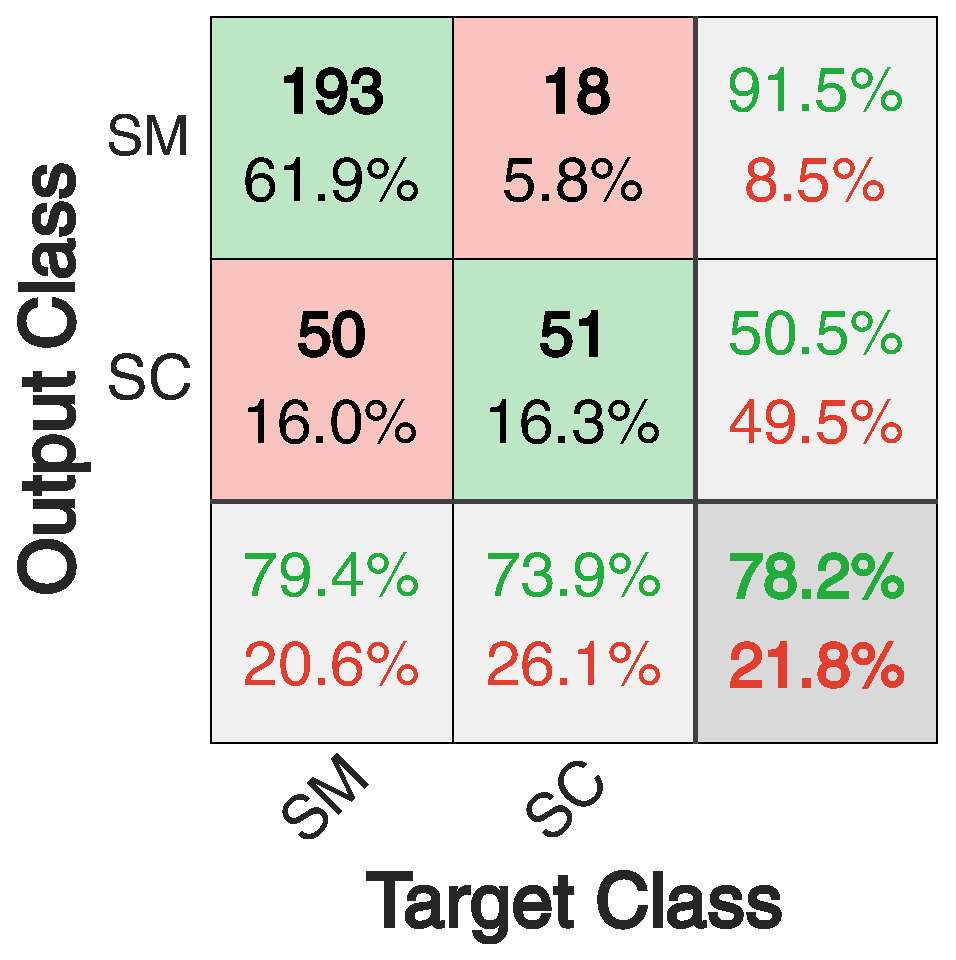
\includegraphics[width=0.3\textwidth]{10m_EffectofMediaCM}
  \caption{Linear support vector machine trained on \emph{catch22} features performed well at classifying cells cultured in complete (SC) and minimal (SM) media.
    Confusion matrix shows one out of ten repeats.
    For each row/column, green numbers indicate the proportion of correct identifications, and red numbers indicate the proportion of incorrect identifications.}
  \label{fig:EffectofMediaCM}
\end{figure}
% Remove top part of figure using Inkscape or something
% ideally I'd generate a figure in which less space is wasted, but I don't have the time now...

\begin{figure}[htbp]
  \centering
  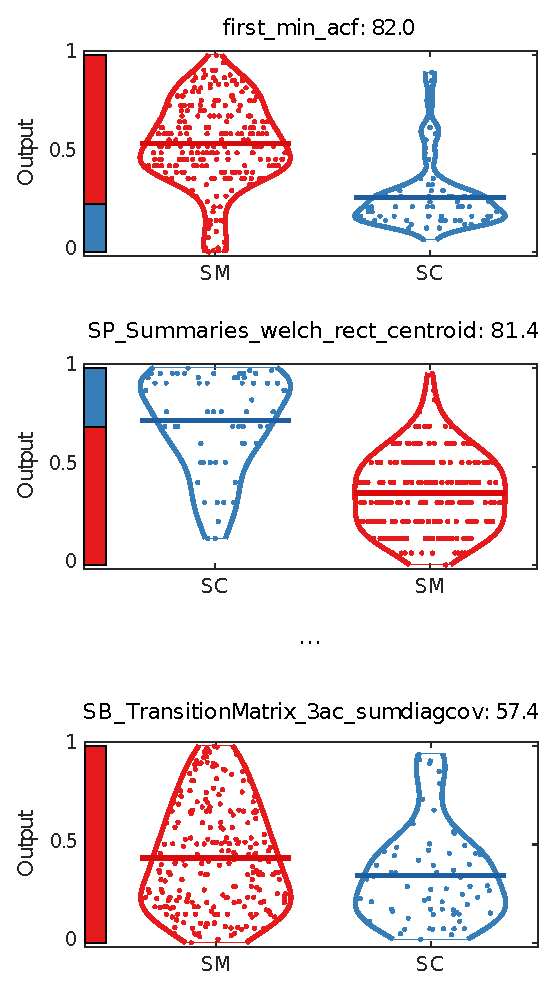
\includegraphics[width=0.45\textwidth]{10m_EffectofMediaTopFeatures}
  \caption{\texttt{first\-Min\_\-acf} and \texttt{SP\_\-Summaries\_\-welch\_\-rect\_\-centroid} performed best at classifying cells cultured in complete and minimal media because the distributions of feature values differed the most between the two groups.
    Numbers above violin plots indicate mean linear classification accuracy.}
  \label{fig:EffectofMediaTopFeatures}
\end{figure}
% might have to crop this

% :: BIG NEW FIGURE ::
\begin{figure}[htbp]
  \centering
  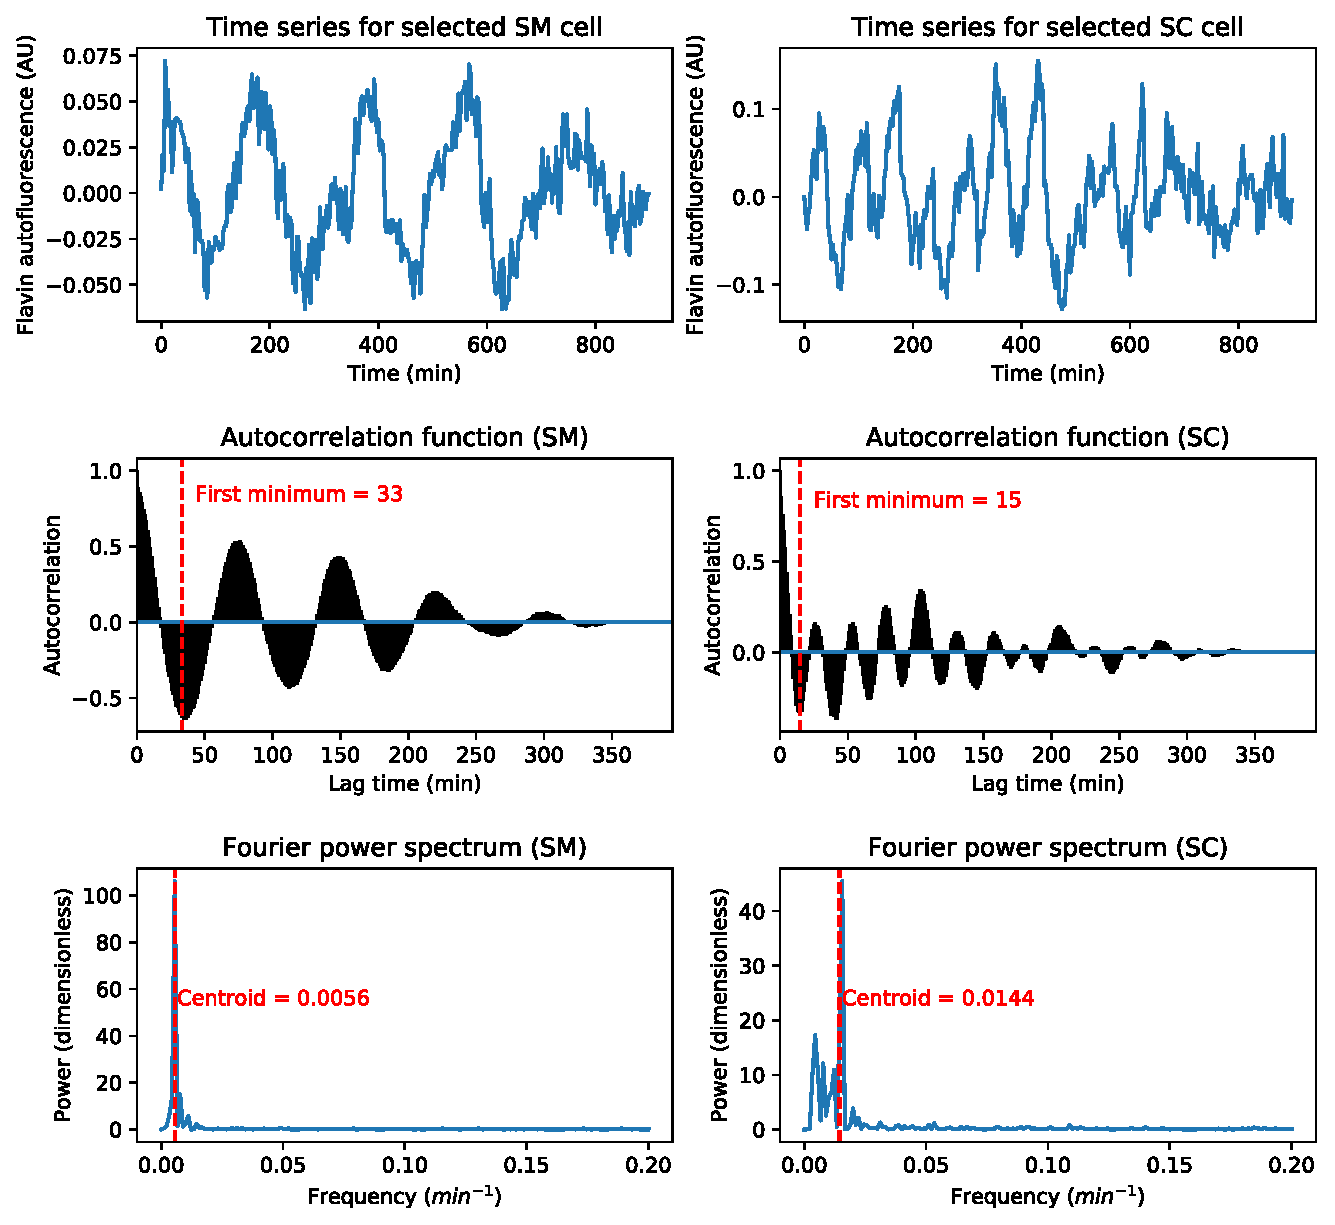
\includegraphics[width=\textwidth]{10m_catch22validation}
  \caption{Comparison of time series, autocorrelation function, and Fourier spectrum for a cell cultured in minimal media (SM) vs a cell cultured in complete media (SC)}
  \label{fig:catch22validation}
\end{figure}

%----- EXPOSURE TIME -----
In contrast, \emph{catch22} features performed poorly at discriminating between the three groups defined by flavin LED exposure time (\SI{60}{\milli\second}, \SI{120}{\milli\second}, \SI{180}{\milli\second}) in the set of cells cultured in complete media (SVM: 32.69\% accuracy, figure \ref{fig:FlavinExpostestCM}; accuracy of random guessing is 33.33\%).
% [I'm not sure if I should include this segue to using full-set hctsa.  I didn't mention it in the oscillating vs non-oscillating section.]
%With the full \emph{hctsa} feature set, the 25 features with the greatest mean linear classification accuracy in discriminating groups defined by exposure time were dependent on mean and spread.
%Having features that best distinguish the groups be dependent on mean and spread was consistent with cells subjected to longer exposure times exhibiting flavin signals of higher intensity %(mean raw readings for \SI{60}{\milli\second}: 0.63 AU, \SI{120}{\milli\second}: 1.3 AU, \SI{180}{\milli\second}: 1.7 AU;
%(standard deviations for time series from \SI{60}{\milli\second}: 0.040 AU, \SI{120}{\milli\second}: 0.067 AU, \SI{180}{\milli\second}: 0.085 AU). % is this needed?  is this too detailed?
These findings suggest that exposure time did not affect the characteristics of flavin autofluorescence traces apart from fluorescence intensity.

\begin{figure}[htbp]
  \centering
  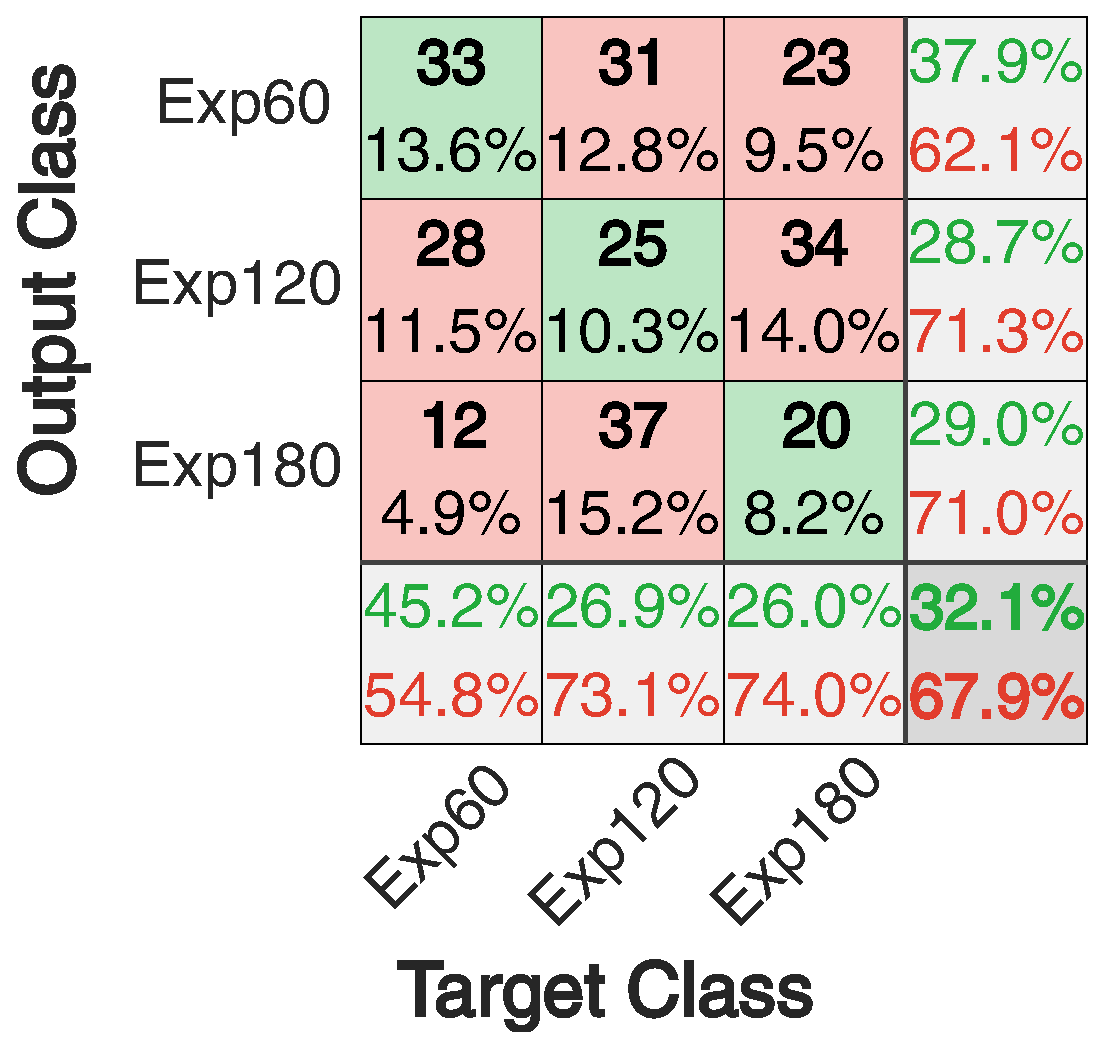
\includegraphics[width=0.4\textwidth]{10m_FlavinExpostestCM}
  \caption{Linear support vector machine trained on \emph{catch22} features performed poorly at classifying cells by LED exposure time.
    Confusion matrix shows one out of ten repeats.
    For each row/column, green numbers indicate the proportion of correct identifications, and red numbers indicate the proportion of incorrect identifications.}
  \label{fig:FlavinExpostestCM}
\end{figure}

%----- OSCILLATING VS NON-OSCILLATING -----

Discrimination between manually-categorised oscillating and non-oscillating flavin autofluorescence traces was also poor (SVM: 66.91\% accuracy, figure \ref{fig:OscillatingCM}; accuracy of random guessing is 50.00\%). %, and using the full \emph{hctsa} feature set was no better (SVM: XX.XX\% accuracy). % Add numbers.  (not sure of violin plots and confusion matrices will be very informative)
These results suggested that using 22 %or even 7700
features across disciplines did not improve on the oscillation classifier (section [INSERT REF HERE]), which was effectively based on one feature, namely, the peak of the normalised classical periodogram.

\begin{figure}[htbp]
  \centering
  \includegraphics[width=0.4\textwidth]{10m_OscillatingCM}
  \caption{Linear support vector machine trained on \emph{catch22} features performed poorly at classifying oscillating and non-oscillating time series.
    Confusion matrix shows one out of ten repeats.
    For each row/column, green numbers indicate the proportion of correct identifications, and red numbers indicate the proportion of incorrect identifications.}
  \label{fig:OscillatingCM}
\end{figure}
